\chapter{Исследовательская часть}

\section{Технические характеристики}

Технические характеристики устройства, на котором выполнялись замеры по времени, представлены далее.

\begin{itemize}
	\item Процессор: Intel(R) Core(TM) i7-1165G7 CPU 2.80 ГГц.
	\item Оперативная память: 15 ГБайт.
	\item Операционная система: Ubuntu 64-разрядная система версии 22.04.3.
\end{itemize}

При замерах времени ноутбук был включен в сеть электропитания и был нагружен только системными приложениями.

\section{Демонстрация работы программы}

На рисунке \ref{img:demonstration} представлена демонстрация работы разработанного программного обеспечения, а именно показаны результаты вычислений реализаций алгоритмов поиска расстояний Левенштейна и Дамерау-Левен-штейна на примере двух строк <<клон>> и <<трон>>.
\clearpage
\begin{figure}[h]
	\centering
	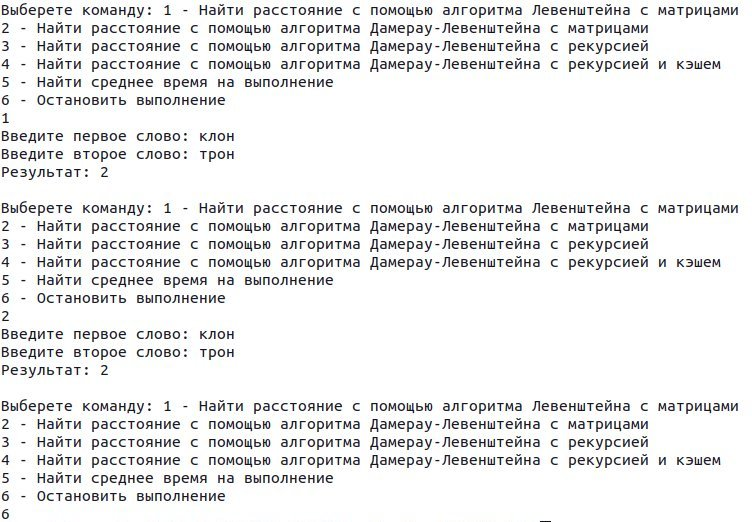
\includegraphics[width=1.0\textwidth, height=0.7\textheight]{img/example.jpg}
	\caption{Демонстрация работы программы при поиске расстояний Левенштейна и Дамерау-Левенштейна}
	\label{img:demonstration}
\end{figure}

\clearpage

\section{Временные характеристики}

Результаты эксперимента замеров по времени приведены в таблице \ref{tbl:time}, в которой есть поля, обозначенные <<\-->>.
Это обусловлено тем, что для рекурсивной реализации алгоритмов достаточно приведенных замеров для построения графика.
По полученным замерам по времени для рекурсивной реализации понятно, что проведения замеров на длин строк больше 9 будет достаточно долгим, поэтому нет смысла проводить замеры по времени рекурсивной реализации алгоритма.
\begin{table}[h]
	\small
	\begin{center}
		\caption{Замер по времени для строк, размер которых от 1 до 200}
		\label{tbl:time}
		\resizebox{\textwidth}{!}{\begin{tabular}{|r|r|r|r|r|}
		\hline
			Кол-во символов & \multicolumn{4}{c|}{Время, мс} \\ \hline
			Длина строки & Левенштейн-Матрица & Дамерау-Левенштейн матрица & Дамерау-Левенштейн рекурсия & Дамерау-Левенштейн рекурсия с кэшем \\ \hline
			1 & 246.100 & 239.000 & 87.700 & 79.100 \\ \hline
			2 & 128.800 & 125.400 & 124.600 & 182.000 \\ \hline
			3 & 263.600 & 267.000 & 734.600 & 297.600 \\ \hline
			4 & 340.600 & 426.400 & 3 664.200 & 498.300 \\ \hline
			5 & 522.200 & 689.200 & 17 661.500 & 723.100 \\ \hline
			6 & 746.500 & 849.400 & 93 846.500 & 1 024.300 \\ \hline
			7 & 1 064.500 & 1 138.300 & 510 799.312 & 1 409.600 \\ \hline
			8 & 1 350.000 & 1 489.400 & 2 901 220.000 & 1 902.600 \\ \hline
			9 & 1 727.500 & 1 880.700 & 16 431 517.000 & 2 401.600 \\ \hline
			10 & 2 106.500 & 2 213.500 & - & 2 879.200 \\ \hline
			20 & 7 065.100 & 7 797.000 & - & 11 505.800 \\ \hline
			30 & 15 460.500 & 17 161.100 & - & 26 226.199 \\ \hline
			40 & 26 836.400 & 29 828.600 & - & 46 470.699 \\ \hline
			50 & 41 745.699 & 49 676.602 & - & 73 213.797 \\ \hline
			60 & 58 991.000 & 65 434.000 & - & 104 228.797 \\ \hline
			70 & 77 570.398 & 86 644.500 & - & 139 459.094 \\ \hline
			80 & 101 191.898 & 113 068.500 & - & 183 324.000 \\ \hline
			90 & 127 196.102 & 142 163.000 & - & 231 846.297 \\ \hline
			100 & 157 460.797 & 174 466.797 & - & 282 203.812 \\ \hline
			200 & 643 454.875 & 711 905.500 & - & 1 158 021.375 \\ \hline
		\end{tabular}}
	\end{center}
\end{table}

Замеры проводились на одинаковых длин строк от 1 до 200 с различным шагом.


Отдельно сравнивается реализации итеративных алгоритмов поиска расстояний Левенштейна и Дамерау--Левенштейна. Сравнение будет производиться на основе данных, представленных в таблице \ref{tbl:time}. Результат можно рассмотреть на рисунке \ref{plt:time_01}.

\begin{figure}[h]
	\centering
	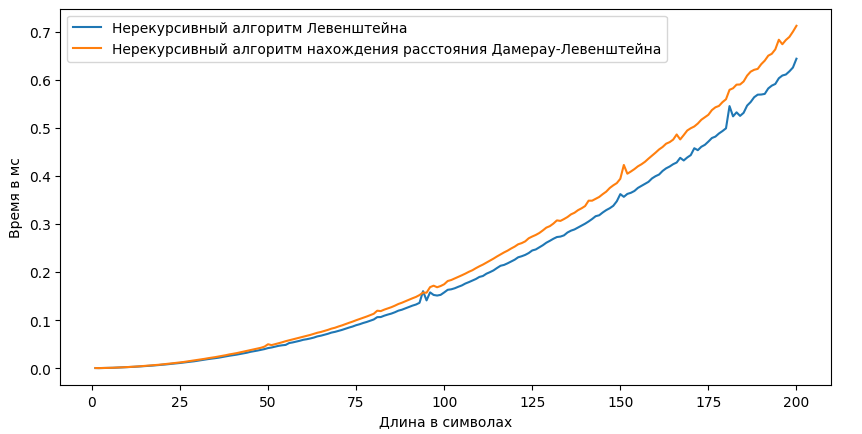
\includegraphics[width=0.8\textwidth]{img/diag_01.png}
	\caption{Сравнение по времени нерекурсивных реализаций алгоритмов поиска расстояний Левенштейна и Дамерау-Левенштейна}
	\label{plt:time_01}
\end{figure}

При длинах строк менее 30 символов разница по времени между итеративными реализациями незначительна, однако при увеличении длины строки алгоритм поиска расстояния Левенштейна затрачивает меньше времени.
Это обосновывается тем, что у алгоритма поиска расстояния Дамерау-Левенштейна задействуется дополнительная операция, которая замедляет алгоритм.

Также сравним рекурсивную и итеративную реализации алгоритма поиска расстояния Дамерау-Левенштейна. Данные представлены в таблице \ref{tbl:time} и отображены на рисунке \ref{plt:time_02}.

\begin{figure}[!htbp]
	\centering
	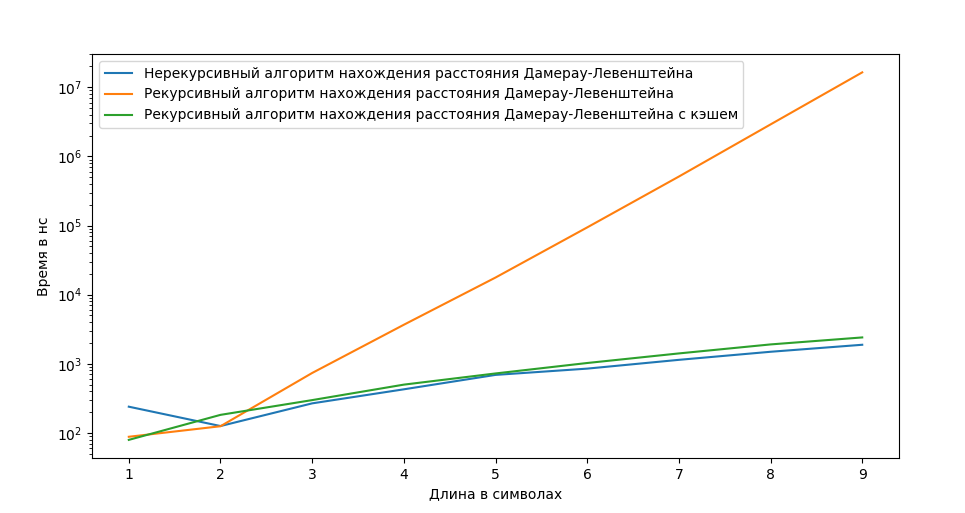
\includegraphics[width=0.9\textwidth]{img/diag_02.png}
	\caption{Сравнение по времени реализаций алгоритмов поиска расстояния Дамерау-Левенштейна}
	\label{plt:time_02}
\end{figure}

На рисунке \ref{plt:time_02} продемонстрировано, что рекурсивный алгоритм без кэширования становится менее эффективным по времени (на 4 порядка больше времени при длине строк равной 8 элементов), чем итеративный и рекурсивный с кэшированием.

Кроме того, согласно данным, приведенным в таблице \ref{tbl:time}, рекурсивный алгоритм без кэширования при длинах строк более 10 элементов не пригодны к использованию в силу экспоненциально роста затрат процессорного времени, в то время, как затраты итеративных алгоритмов и рекурсивного алгоритма с кэшированием по времени линейны.

\section{Характеристики по памяти}

Введем следующие обозначения:
\begin{itemize}
	\item$n$ --- длина строки $S_{1}$;
	\item$m$ --- длина строки $S_{2}$;
	\item$size()$ --- функция вычисляющая размер в байтах;
	\item $string$ --- строковый тип;
	\item $int$ --- целочисленный тип;
	\item $size\_t$ --- беззнаковый целочисленный тип.
\end{itemize}

Максимальная глубина стека вызовов при рекурсивной реализации нахождения расстояния Дамерау-Левенштейна равна сумме входящих строк, а на каждый вызов требуется 2 дополнительные переменные, соответственно, максимальный расход памяти вычисляется по формуле:
\begin{equation}
	\label{eq:dl_rec_memory}
	(n + m) \cdot (2 \cdot size(string) + 3 \cdot size(int) + 2 \cdot sizeof(size\_t)),
\end{equation}
где:
\begin{itemize}
	\item $2 \cdot size(string)$ --- хранение двух строк;
	\item $2 \cdot size(size\_t)$ --- хранение размеров строк;
	\item $2 \cdot size(int)$ --- дополнительные переменные;
	\item $size(int)$ --- адрес возврата.
\end{itemize}

Для рекурсивного алгоритма c кешированием поиска расстояния Да-мерау-Левенштейна будет теоретически схож с расчетом в формуле (\ref{eq:dl_rec_memory}), но также учитывается матрица, соответственно, максимальный расход памяти вычисляется по формуле:
\begin{equation}
	\label{eq:dl_hash_memory}
	\begin{aligned}
		(n + m) \cdot (2 \cdot size(string) + 3 \cdot size(int) + 2 \cdot size(size\_t)) + \\
		+ (n + 1) \cdot (m + 1) \cdot size(int).
	\end{aligned}
\end{equation}
Использование памяти при итеративной реализации алгоритма поиска расстояния Левенштейна теоретически вычисляется по формуле:
\begin{equation}
	\label{eq:lev_mtr_memory}
	\begin{aligned}
		(n + 1) \cdot (m + 1) \cdot size(int) + 2 \cdot size(string) + 2 \cdot size(size\_t) + \\
		+ size(int **) + (n + 1) \cdot size(int *) + 2 \cdot size(int),
	\end{aligned}
\end{equation}
где
\begin{itemize}
	\item $2 \cdot size(string)$ --- хранение двух строк;
	\item $2 \cdot size(size\_t)$ --- хранение размеров матрицы;
	\item $(n + 1) \cdot (m + 1) \cdot size(int)$ --- хранение матрицы;
	\item $size(int **) + (n + 1) \cdot size(int *)$ --- указатель на матрицу;
	\item $size(int)$ --- дополнительная переменная для хранения результата;
	\item $size(int)$ --- адрес возврата.
\end{itemize}

Использование памяти при итеративной реализации алгоритма поиска расстояния Дамерау-Левенштейна теоретически вычисляется по формуле:
\begin{equation}
	\label{eq:dl_mtr_memory}
	\begin{aligned}
		(n + 1) \cdot (m + 1) \cdot size(int) + 2 \cdot size(string) + 2 \cdot size(size\_t) + \\
		+ size(int **) + (n + 1) \cdot size(int *) + 3 \cdot size(int),
	\end{aligned}
\end{equation}
где
\begin{itemize}
	\item $2 * size(string)$ --- хранение двух строк;
	\item $2 \cdot size(size\_t)$ --- хранение размеров матрицы;
	\item $(n + 1) \cdot (m + 1) \cdot size(int)$ --- хранение матрицы;
	\item $size(int **) + (n + 1) \cdot size(int *)$ --- указатель на матрицу;
	\item $2 \cdot size(int)$ --- дополнительные переменные;
	\item $size(int)$ --- адрес возврата.
\end{itemize}

По расходу памяти итеративные алгоритмы проигрывают рекурсивным: максимальный размер используемой памяти в итеративном растет как произведение длин строк, в то время как у рекурсивного алгоритма — как сумма длин строк.

По формулам \ref{eq:dl_rec_memory} -- \ref{eq:lev_mtr_memory} затрат по памяти в программе были написаны соответствующие функции для подсчета расходуемой памяти, результаты расчетов, которых представлены в таблице \ref{tbl:memory}, где размеры строк находятся в диапазоне от 10 до 200 с шагом 10.

\begin{table}[!ht]
    \centering
	\small
	\begin{center}
		\caption{Замер памяти для строк, размером от 10 до 200}
		\label{tbl:memory}
		\resizebox{0.6\textwidth}{!}{\begin{tabular}{|r|r|r|r|r|}
		\hline
			Len & lev & dl & dl\_rec & dl\_rec\_cash \\ \hline
			10 & 668 & 672 & 1 840 & 2 420 \\ \hline
			20 & 2 028 & 2 032 & 3 680 & 5 620 \\ \hline
			30 & 4 188 & 4 192 & 5 520 & 9 620 \\ \hline
			40 & 7 148 & 7 152 & 7 360 & 14 420 \\ \hline
			50 & 10 908 & 10 912 & 9 200 & 20 020 \\ \hline
			60 & 15 468 & 15 472 & 11 040 & 26 420 \\ \hline
			70 & 20 828 & 20 832 & 12 880 & 33 620 \\ \hline
			80 & 26 988 & 26 992 & 14 720 & 41 620 \\ \hline
			90 & 33 948 & 33 952 & 16 560 & 50 420 \\ \hline
			100 & 41 708 & 41 712 & 18 400 & 60 020 \\ \hline
			110 & 50 268 & 50 272 & 20 240 & 70 420 \\ \hline
			120 & 59 628 & 59 632 & 22 080 & 81 620 \\ \hline
			130 & 69 788 & 69 792 & 23 920 & 93 620 \\ \hline
			140 & 80 748 & 80 752 & 25 760 & 106 420 \\ \hline
			150 & 92 508 & 92 512 & 27 600 & 120 020 \\ \hline
			160 & 105 068 & 105 072 & 29 440 & 134 420 \\ \hline
			170 & 118 428 & 118 432 & 31 280 & 149 620 \\ \hline
			180 & 132 588 & 132 592 & 33 120 & 165 620 \\ \hline
			190 & 147 548 & 147 552 & 34 960 & 182 420 \\ \hline
			200 & 163 308 & 163 312 & 36 800 & 200 020 \\ \hline
		\end{tabular}}
	\end{center}
\end{table}

\clearpage

Из данных, приведенных в таблице \ref{tbl:memory}, понятно, что рекурсивные алгоритмы являются более эффективными по памяти, так как используется только память под локальные переменные, передаваемые аргументы и возвращаемое значение, в то время как итеративные алгоритмы затрачивают память линейно пропорционально длинам обрабатываемых строк.

\begin{figure}[!htbp]
	\centering
	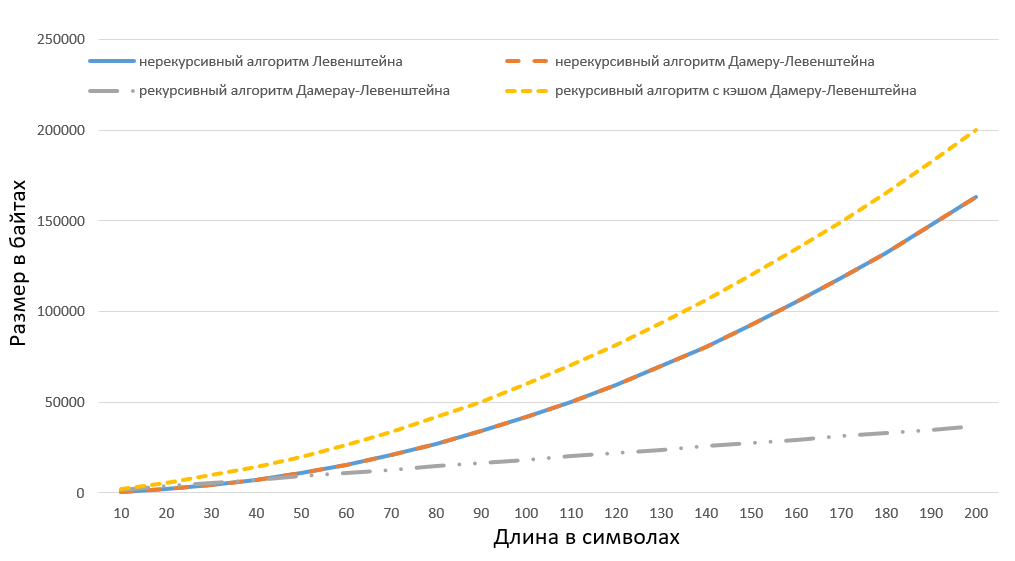
\includegraphics[width=\textwidth]{img/diag_03.png}
	\caption{Сравнение по памяти реализаций алгоритмов поиска расстояния Левенштейна и Дамерау-Левенштейна --- итеративной и рекурсивной реализации}
	\label{plt:memory}
\end{figure}

Из рисунка \ref{plt:memory_1} понятно, что рекурсивная реализация алгоритма поиска расстояния Дамерау-Левенштейна более эффективна по памяти, чем итеративная.

\begin{figure}[!htbp]
	\centering
	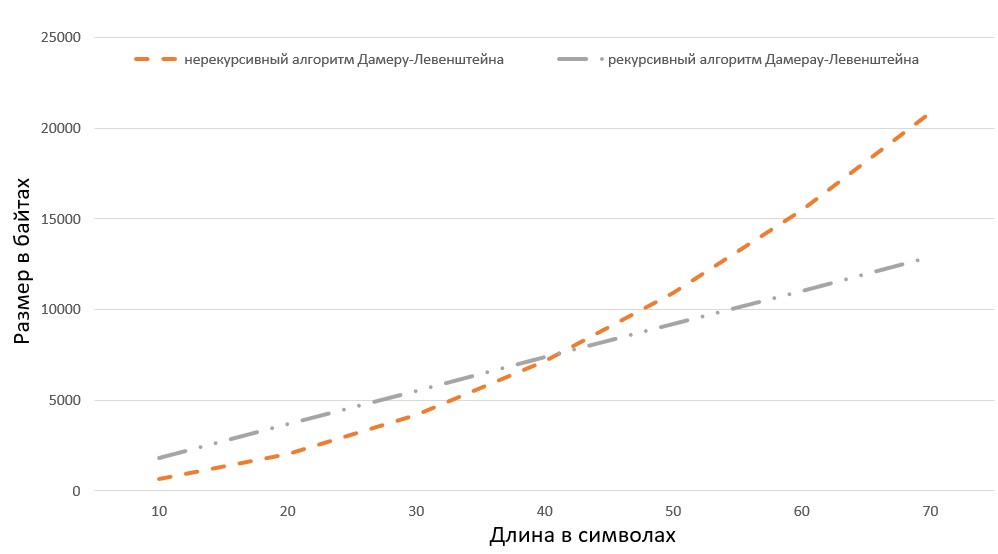
\includegraphics[width=\textwidth]{img/diag_04.png}
	\caption{Сравнение по памяти реализаций алгоритмов поиска расстояния Дамерау-Левенштейна --- итеративной и рекурсивной реализации}
	\label{plt:memory_1}
\end{figure}

\clearpage

\section{Вывод}

В данном разделе было произведено сравнение количества затраченного времени и памяти реализаций алгоритмов поиска расстояний Левенштейна и Дамерау-Левенштейна.
Наименее затратным по времени оказалась итеративная реализация алгоритма нахождения расстояния Левенштейна.
Наименее затратным по памяти оказался рекурсивный алгоритм нахождения расстояния Дамерау-Левенштейна.

Приведенные характеристики показывают, что рекурсивная реализация алгоритма поиска расстояния Дамерау-Левенштейна в 30 раз проигрывает по времени итеративной реализации при строках длиной 5, однако выигрывает по памяти в 5 раз при строках длиной 200.
Несмотря на выигрыш по памяти при росте длины строки по сравнению с нерекурсивным алгоритмом, рекурсивный алгоритм следует использовать лишь для малых размерностей строк (1 -- 4 символа), так как рост времени на выполнение делает его неприменимым для более длинных строк.

Написанная реализация рекурсивного алгоритма поиска расстояния Дамерау-Левенштейна с кэшированием проигрывает нерекурсивной реализации по времени при всех строках, длина которых больше 1, и всегда проигрывает по памяти.
Из этого можно сделать вывод, что нерекурсивный алгоритм поиска расстояния Дамерау-Левенштейна стоит использовать вместо рекурсивных реализаций во всех рассмотренных случаях.

Сравнивая нерекурсивные алгоритмы поиска расстояния Левенштейна и Дамерау-Левенштейна, стоит учесть, что во время печати очень часто возникают ошибки, связанные с транспозицией букв, из-за чего для поиска меры разницы двух строк стоит использовать алгоритмы поиска расстояния Дамерау-Левенштейна, несмотря на то, что приведенные реализации алгоритмов либо требуют больше времени, либо используют больше памяти, чем представленная реализация алгоритма поиска расстояния Левенштейна.
